\documentclass[11pt]{article}
\usepackage[margin=1in]{geometry}
\usepackage{amsmath,amssymb}
\usepackage{tikz}
\usetikzlibrary{arrows.meta}
\usepackage{booktabs}

\title{Column Generation for Max Flow (Path Formulation)}
\author{}
\date{}

\begin{document}
\maketitle

\section{Formulation}
Let $G=(V,A)$ be a directed graph with source $s$, sink $t$, and arc capacities $u_a$. Let $\mathcal{P}$ be the set of all $s$--$t$ paths and $f_p\ge 0$ the flow on path $p$.

\textbf{Master problem:}
\begin{align*}
\max\quad & \sum_{p\in\mathcal{P}} f_p\\
\text{s.t.}\quad & \sum_{p\in\mathcal{P}:\,a\in p} f_p \le u_a && \forall a\in A \quad [\text{dual } y_a\ge 0]\\
& f_p\ge 0 && \forall p\in\mathcal{P}
\end{align*}

\textbf{Restricted master problem (RMP):} the same problem, but with only a subset $\mathcal{P}'\subseteq\mathcal{P}$ of paths:
\begin{align*}
\max\quad & \sum_{p\in\mathcal{P}'} f_p\\
\text{s.t.}\quad & \sum_{p\in\mathcal{P}':\,a\in p} f_p \le u_a && \forall a\in A \quad [\text{dual } y_a\ge 0]\\
& f_p\ge 0 && \forall p\in\mathcal{P}'
\end{align*}
The RMP has the same constraints (one per arc) but fewer variables (columns). Any RMP solution is a feasible flow for the MP, with the missing paths set to $0$.

\textbf{Why use the RMP?} The number of $s$--$t$ paths can grow exponentially with the size of the network, so the full master problem is too large to write down and solve. The RMP is small enough to solve directly. Its duals $y_a^*$ tell us how valuable each unit of arc capacity currently is, and the pricing problem uses them to find the one missing path most worth adding. Repeating this grows the RMP only as far as needed, until it has the same optimal value as the full master problem.

\section{Duals, Reduced Cost, and Pricing}
\textbf{Duals as prices.} Each capacity constraint of the RMP has a dual value $y_a\ge 0$. It is the \emph{shadow price} of arc $a$: the gain in the flow value per extra unit of capacity $u_a$ (that is, $\Delta z/\Delta u_a$, valid for small changes). An arc with slack capacity has $y_a=0$. The duals of a maximum flow mark the arcs of a minimum cut.

\textbf{Cost and benefit of a path.} Sending one unit of flow along path $p$
\begin{itemize}
  \item \emph{earns} $1$ unit of flow (its objective coefficient), and
  \item \emph{costs} $\sum_{a\in p} y_a^*$, since it uses one unit of capacity on every arc of the path, each valued at its dual price.
\end{itemize}

\textbf{Reduced cost.} The reduced cost of path $p$ is the benefit minus the cost:
\[
\bar c_p \;=\; 1-\sum_{a\in p} y_a^* .
\]
\begin{center}
\small
\begin{tabular}{@{}lll@{}}
\toprule
Path cost $\sum_{a\in p}y^*_a$ & Reduced cost $\bar c_p$ & Meaning \\
\midrule
$<1$ & $>0$ & Earns more than it costs: adding it raises the flow. \\
$=1$ & $=0$ & Break-even: no gain from adding it. \\
$>1$ & $<0$ & Costs more than it earns: adding it would not help. \\
\bottomrule
\end{tabular}
\end{center}

\textbf{Pricing problem.} A missing path helps only if $\bar c_p>0$. Since the earning of every path is the constant $1$, maximizing $\bar c_p$ is the same as minimizing the path cost:
\[
\min_{p\in\mathcal{P}} \sum_{a\in p} y_a^* .
\]
This is a shortest $s$--$t$ path problem in which the \emph{duals are the arc costs}. These costs are re-priced from the RMP every iteration. Arcs with spare capacity cost $0$, so the shortest path is drawn toward unused capacity, while saturated bottleneck arcs cost more and are avoided. Because $y_a^*\ge 0$, Dijkstra's algorithm applies.

\textbf{Stopping rule.} If the shortest path has cost $\ge 1$, then $\bar c_p\le 0$ for every path, so no missing column can improve the objective and the RMP solution is optimal for the MP.

\section{The Algorithm in Words}
Start with a small set of paths, for example a single $s$--$t$ path. Solve the restricted master problem and read off the dual value $y_a$ of each capacity constraint. Use these as arc lengths and find the shortest path from $s$ to $t$. If its length is less than $1$, this path can increase the flow, so add it to the set and solve the restricted master again. If its length is at least $1$, no missing path can help, so the current flow is a maximum flow. Its value equals the capacity of a minimum cut, which is given by the final duals.

\section{Example on a 6-Node Network}
\begin{figure}[h]
\centering
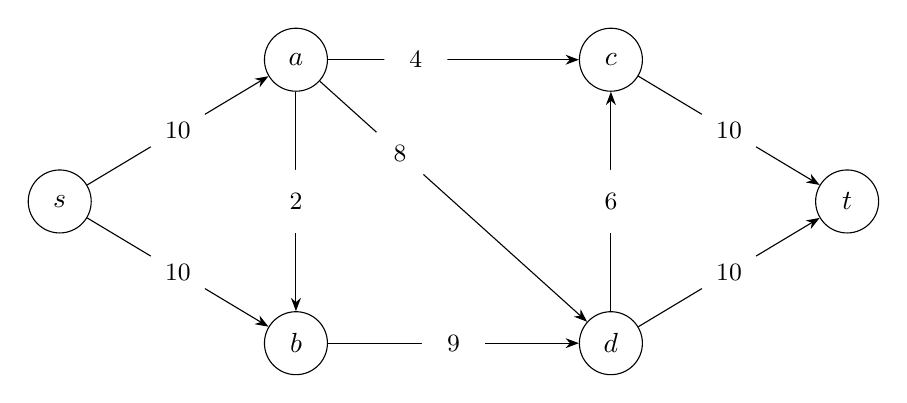
\begin{tikzpicture}[>=Stealth,
  every node/.style={circle,draw,minimum size=8mm,inner sep=0pt},
  lab/.style={draw=none,fill=white,inner sep=1pt,font=\small}]
  \node (s) at (0,0) {$s$};
  \node (a) at (3,1.8) {$a$};
  \node (b) at (3,-1.8) {$b$};
  \node (c) at (7,1.8) {$c$};
  \node (d) at (7,-1.8) {$d$};
  \node (t) at (10,0) {$t$};
  \draw[->] (s) -- node[lab] {10} (a);
  \draw[->] (s) -- node[lab] {10} (b);
  \draw[->] (a) -- node[lab] {2} (b);
  \draw[->] (a) -- node[lab,pos=0.35] {4} (c);
  \draw[->] (a) -- node[lab,pos=0.3] {8} (d);
  \draw[->] (b) -- node[lab] {9} (d);
  \draw[->] (d) -- node[lab] {6} (c);
  \draw[->] (c) -- node[lab] {10} (t);
  \draw[->] (d) -- node[lab] {10} (t);
\end{tikzpicture}
\caption{Example network with arc capacities.}
\end{figure}

The network has seven $s$--$t$ paths:
$P_1=s\to a\to c\to t$,\; $P_2=s\to a\to d\to t$,\; $P_3=s\to b\to d\to t$,\; $P_4=s\to a\to d\to c\to t$,\; $P_5=s\to a\to b\to d\to t$,\; $P_6=s\to a\to b\to d\to c\to t$,\; $P_7=s\to b\to d\to c\to t$.
We start with $\mathcal{P}'=\{P_1\}$ and add paths as pricing finds them.

\textbf{Table 1: RMP results and all duals.} Each row lists the RMP optimum and the dual value $y^*_a$ of every arc, including the zeros.
\begin{center}
\footnotesize
\setlength{\tabcolsep}{3.5pt}
\begin{tabular}{@{}cllcccccccccc@{}}
\toprule
 & & & \multicolumn{9}{c}{Dual $y^*_a$ of arc} & \\
\cmidrule(lr){4-12}
It. & $\mathcal{P}'$ & Obj. & $sa$ & $sb$ & $ab$ & $ac$ & $ad$ & $bd$ & $dc$ & $ct$ & $dt$ & Added \\
\midrule
1 & $P_1$ & 4 & 0 & 0 & 0 & \textbf{1} & 0 & 0 & 0 & 0 & 0 & $P_2$ \\
2 & $P_1,P_2$ & 10 & \textbf{1} & 0 & 0 & 0 & 0 & 0 & 0 & 0 & 0 & $P_3$ \\
3 & $P_1,P_2,P_3$ & 14 & 0 & 0 & 0 & \textbf{1} & 0 & 0 & 0 & 0 & \textbf{1} & $P_4$ \\
4 & $P_1,\dots,P_4$ & 19 & \textbf{1} & 0 & 0 & 0 & 0 & \textbf{1} & 0 & 0 & 0 & none \\
\bottomrule
\end{tabular}
\end{center}

\textbf{Table 2: Path cost and reduced cost.} For each path, the entry is its cost $\sum_{a\in p}y^*_a$ under that row's duals, followed by its reduced cost $\bar c_p = 1-\text{cost}$. A path is a candidate when $\bar c_p>0$.
\begin{center}
\footnotesize
\setlength{\tabcolsep}{4pt}
\begin{tabular}{@{}cccccccc@{}}
\toprule
It. & $P_1$ & $P_2$ & $P_3$ & $P_4$ & $P_5$ & $P_6$ & $P_7$ \\
\midrule
1 & 1 / 0 & \textbf{0 / 1} & 0 / 1 & 0 / 1 & 0 / 1 & 0 / 1 & 0 / 1 \\
2 & 1 / 0 & 1 / 0 & \textbf{0 / 1} & 1 / 0 & 1 / 0 & 1 / 0 & 0 / 1 \\
3 & 1 / 0 & 1 / 0 & 1 / 0 & \textbf{0 / 1} & 1 / 0 & 0 / 1 & 0 / 1 \\
4 & 1 / 0 & 1 / 0 & 1 / 0 & 1 / 0 & 2 / $-1$ & 2 / $-1$ & 1 / 0 \\
\bottomrule
\end{tabular}
\end{center}
Entries are ``cost / reduced cost''; the bold entry is the path added that iteration. Several paths tie at reduced cost $1$ in iterations 1--3, and the shortest path routine returns one of them.

\textbf{Reading the tables.} Pricing adds a path whose \emph{total} cost is below $1$, not an arc whose dual happens to be $0$. The largest possible reduced cost is $1$, reached by a path whose arcs all have dual $0$, that is, a path through arcs with spare capacity. That is why the paths added in iterations 1--3 have cost $0$: they are the paths with the highest reduced cost. A path with a few small positive duals could also be below $1$. Once a path is added, the duals are re-priced, and the added path's reduced cost drops to $0$ (iterations 2--4 show $P_2$, $P_3$, $P_4$ at cost $1$). In iteration 4 no path has reduced cost above $0$, so the algorithm stops.

At iteration 4 the shortest path has length $1$, so the algorithm stops. The maximum flow is $19$. The final duals mark the minimum cut $\{(s,a),(b,d)\}$ with capacity $10+9=19$.

\end{document}
